\documentclass{article}
\usepackage{xcolor}
\usepackage{titleps}
\usepackage[letterpaper, margin=0.95in]{geometry}
\usepackage{url}
\usepackage{amsmath}
\usepackage{amssymb}
\usepackage{wrapfig}
\usepackage{float}
\usepackage{mathtools}
\usepackage{enumitem}
\usepackage{tabu}
\usepackage{parskip}
\usepackage{natbib}
\usepackage{listings}

\usepackage[many]{tcolorbox}
\usepackage{minted}
\setminted[python]{
	% frame=single,
	% linenos,
    xleftmargin=0.475em,
    baselinestretch=1.2,
}
% https://tex.stackexchange.com/a/569249
\setcounter{secnumdepth}{5}
\setcounter{tocdepth}{5}
\makeatletter
\newcommand\subsubsubsection{\@startsection{paragraph}{4}{\z@}{-2.5ex\@plus -1ex \@minus -.25ex}{1.25ex \@plus .25ex}{\normalfont\normalsize\bfseries}}
\newcommand\subsubsubsubsection{\@startsection{subparagraph}{5}{\z@}{-2.5ex\@plus -1ex \@minus -.25ex}{1.25ex \@plus .25ex}{\normalfont\normalsize\bfseries}}
\makeatother

\usepackage{hyperref}
\usepackage[color=red]{todonotes}
\usepackage{forest}
\definecolor{light-yellow}{HTML}{FFE5CC}

\newpagestyle{ruled}
{\sethead{CMU 16-831}{Introduction to Robot Learning }{Fall 2026}\headrule
  \setfoot{}{}{}}
\pagestyle{ruled}

\renewcommand\makeheadrule{\color{black}\rule[-.75\baselineskip]{\linewidth}{0.4pt}}
\renewcommand*\footnoterule{}

\newtcolorbox[]{answer}[1][]{
    % breakable,
    enhanced,
    nobeforeafter,
    colback=white,
    title=Your Answer,
    sidebyside align=top,
    box align=top,
    #1
}



\begin{document}

\lstset{basicstyle = \ttfamily,columns=fullflexible,
backgroundcolor = \color{light-yellow}
}

\begin{centering}
    {\Large Assignment 2: Policy Gradient} \\
    \vspace{.25cm}
    % \textbf{Due September 13, 11:59 pm} \\
\end{centering}
\vspace{0.25cm}

\textbf{Andrew ID:} \texttt{ncheng2} \\
\textbf{Collaborators:} \texttt{None.}\\ 
\textbf{NOTE:} Please do \textbf{NOT} change the sizes of the answer blocks or plots.

\setcounter{section}{4}
\section{Small-Scale Experiments (7.5 Pts)}

\subsection{Experiment 1 (Cartpole) -- \lbrack4.5 points total\rbrack}

\subsubsection{Configurations}
\begin{answer}[title=Q5.1.1,height=6cm,width=\linewidth]
\begin{minted}[framesep=2mm, fontsize=\scriptsize, breaklines]{bash}
python -m rob831.scripts.run_hw2 --env_name CartPole-v0 -n 150 -b 1500 \
    -dsa --exp_name q1_sb_no_rtg_dsa
python -m rob831.scripts.run_hw2 --env_name CartPole-v0 -n 150 -b 1500 \
    -rtg -dsa --exp_name q1_sb_rtg_dsa
python -m rob831.scripts.run_hw2 --env_name CartPole-v0 -n 150 -b 1500 \
    -rtg --exp_name q1_sb_rtg_na
python -m rob831.scripts.run_hw2 --env_name CartPole-v0 -n 150 -b 6000 \
    -dsa --exp_name q1_lb_no_rtg_dsa
python -m rob831.scripts.run_hw2 --env_name CartPole-v0 -n 150 -b 6000 \
    -rtg -dsa --exp_name q1_lb_rtg_dsa
python -m rob831.scripts.run_hw2 --env_name CartPole-v0 -n 150 -b 6000 \
    -rtg --exp_name q1_lb_rtg_na
\end{minted}
\end{answer}

\subsubsection{Plots}

\subsubsubsection{Small batch -- \lbrack1 points\rbrack}
\begin{answer}[title=Q5.1.2.1,height=9.5cm,width=\linewidth]
\centering
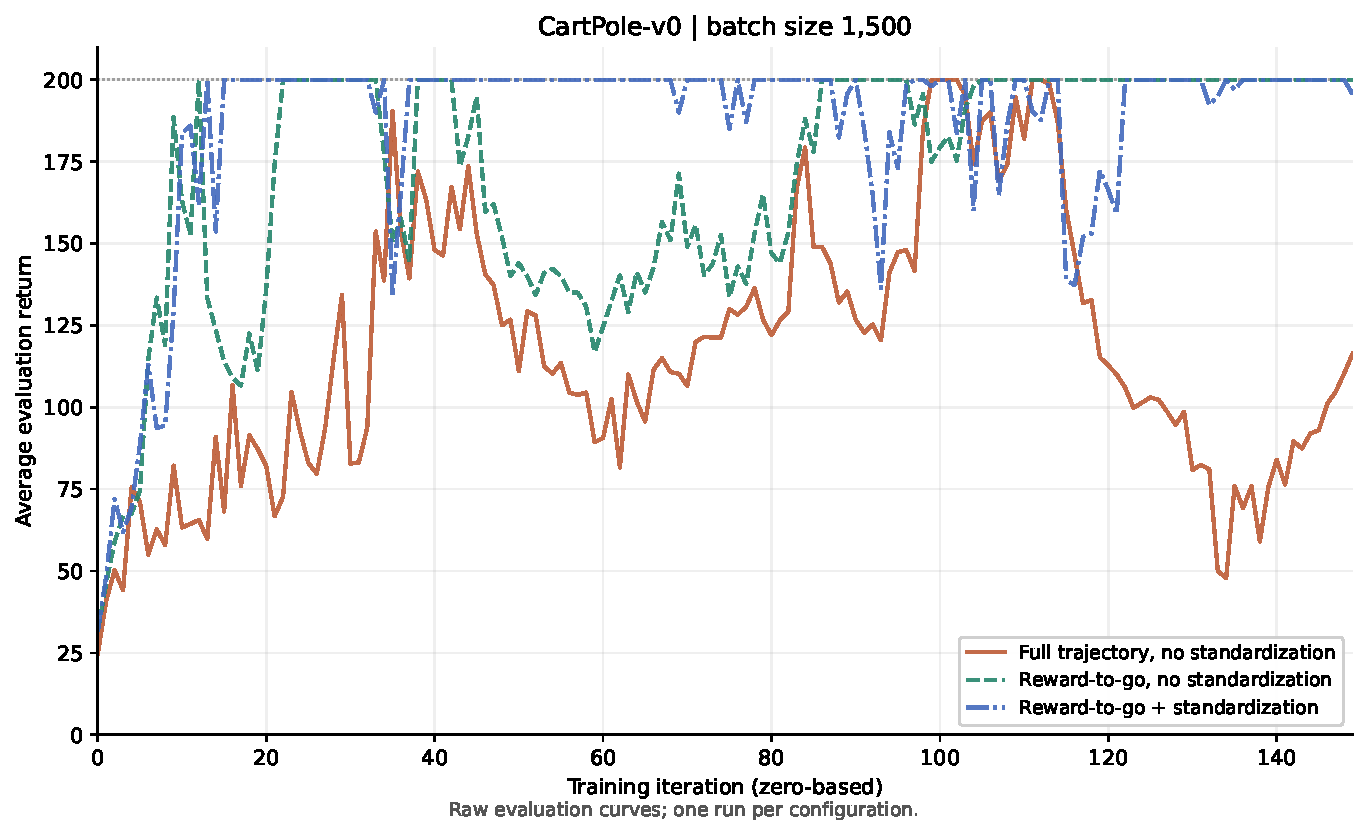
\includegraphics[height=8cm]{results/q1/q1_sb.pdf}
\end{answer}

\subsubsubsection{Large batch -- \lbrack0.5 points\rbrack}
\begin{answer}[title=Q5.1.2.2,height=9.5cm,width=\linewidth]
\centering
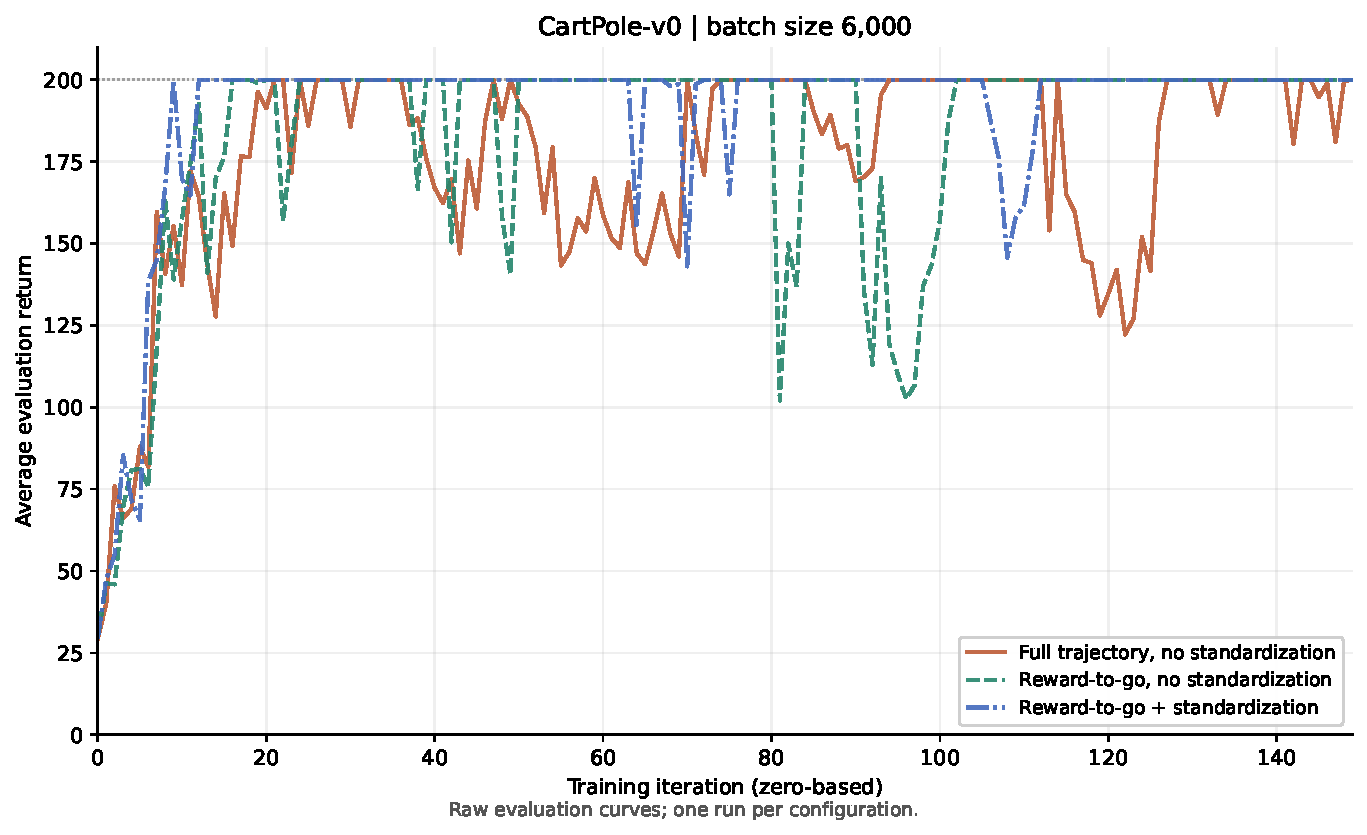
\includegraphics[height=8cm]{results/q1/q1_lb.pdf}
\end{answer}

\subsubsection{Analysis}

\subsubsubsection{Value estimator -- \lbrack1 points\rbrack}
\begin{answer}[title=Q5.1.3.1,height=4cm,width=\linewidth]
Without advantage standardization, reward-to-go performed better, especially
with the small batch. The mean evaluation returns over the last 20 iterations
were 82.60 (full trajectory) versus 200.00 (reward-to-go) for batch size 1500,
and 197.20 versus 200.00 for batch size 6000. Reward-to-go excludes rewards
received before the action and thus removes irrelevant past-reward terms from the
gradient estimator, reducing its variance.
\end{answer}

\subsubsubsection{Advantage standardization -- \lbrack1 points\rbrack}
\begin{answer}[title=Q5.1.3.2,height=4cm,width=\linewidth]
Standardization improved early learning in these runs but final performance 
was similar.
Centering and scaling advantages makes updates less
sensitive to the return scale.
\end{answer}

\subsubsubsection{Batch size -- \lbrack1 points\rbrack}
\begin{answer}[title=Q5.1.3.3,height=4cm,width=\linewidth]
Increasing the batch size from 1500 to 6000 helped the full-trajectory
estimator most. Larger batches average over
more trajectories and can reduce sampling noise, but require more environment steps and time per update.
\end{answer}

\subsection{Experiment 2 (InvertedPendulum) -- \lbrack3 points total\rbrack}

\subsubsection{Configurations -- \lbrack1 points\rbrack}
\begin{answer}[title=Q5.2.1,height=10cm,width=\linewidth]
\begin{minted}[framesep=2mm, fontsize=\scriptsize, breaklines]{bash}
export OMP_NUM_THREADS=1 MKL_NUM_THREADS=1 OPENBLAS_NUM_THREADS=1
# All 15 new search configurations; seed 1 (default).
for spec in "50 0.01" "50 0.02" "50 0.03" "50 0.04" "50 0.05" \
            "100 0.01" "100 0.02" "100 0.03" "100 0.04" "100 0.05" \
            "200 0.01" "200 0.02" "200 0.03" "200 0.1" "500 0.05"; do
  read -r b r <<< "$spec"
  python -m rob831.scripts.run_hw2 --env_name InvertedPendulum-v4 \
    --ep_len 1000 --discount 0.92 -n 100 -l 2 -s 64 \
    -b "$b" -lr "$r" -rtg --no_gpu --exp_name "q2_b${b}_r${r}"
done
\end{minted}
Two pre-existing runs ($b=500,1000$, $r=0.01$) were also inspected.
New runs used the activated homework Conda environment and CPU execution;
all other arguments retain their defaults (seed 1, evaluation batch 400,
video logging disabled). All search runs completed 100 iterations.
\end{answer}

\subsubsection{smallest \textbf{b*} and largest \textbf{r*} (same run) -- \lbrack1 points\rbrack}
\begin{answer}[title=Q5.2.2,height=4cm,width=\linewidth]
\small
Among tested configurations, the smallest batch reaching 1000 was
$\mathbf{b^*=50}$; its largest tested successful rate was
$\mathbf{r^*=0.03}$ in the same run. It first reached 1000 at iteration 53
(zero-based), with 20 evaluations at 1000, but its final return was 106
and last-10 mean was 444.65. For a more stable alternative, $b=100,r=0.03$
first reached 1000 at iteration 65 and stayed at 1000 for the final 10
iterations. Both curves are shown below. This finite, single-seed search
establishes tested outcomes, not global extrema; a batch target is a minimum
because complete trajectories are collected.
\end{answer}

\subsubsection{Plot -- \lbrack1 points\rbrack}
\begin{answer}[title=Q5.2.3,height=10cm,width=\linewidth]
\centering
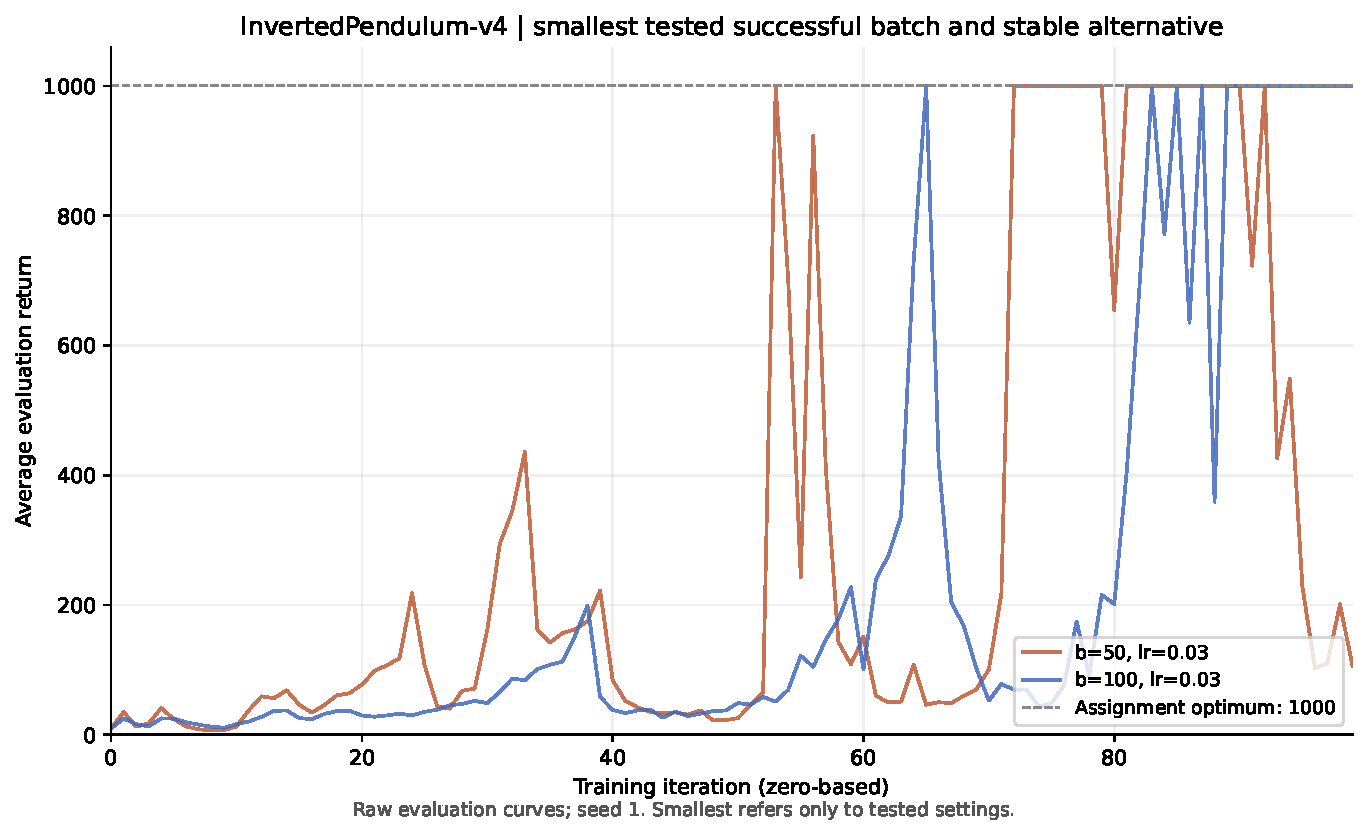
\includegraphics[height=8cm]{results/q2/q2_comparison.pdf}
\end{answer}

\setcounter{section}{6}
\section{More Complex Experiments (4.5 Pts)}

\subsection{Experiment 3 (LunarLander) -- \lbrack1 points total\rbrack}

\subsubsection{Configurations}
\begin{answer}[title=Q7.1.1,height=6cm,width=\linewidth]
\begin{minted}
[framesep=2mm, fontsize=\scriptsize, breaklines]
{bash}
python -m rob831.scripts.run_hw2 \
    --env_name LunarLanderContinuous-v2 --ep_len 1000 \
    --discount 0.99 -n 100 -l 2 -s 64 -b 10000 -lr 0.005 \
    --reward_to_go --nn_baseline --exp_name q3_b10000_r0.005
\end{minted}
\end{answer}

\subsubsection{Plot -- \lbrack1 points\rbrack}
\begin{answer}[title=Q7.1.2,height=10cm,width=\linewidth]
\centering
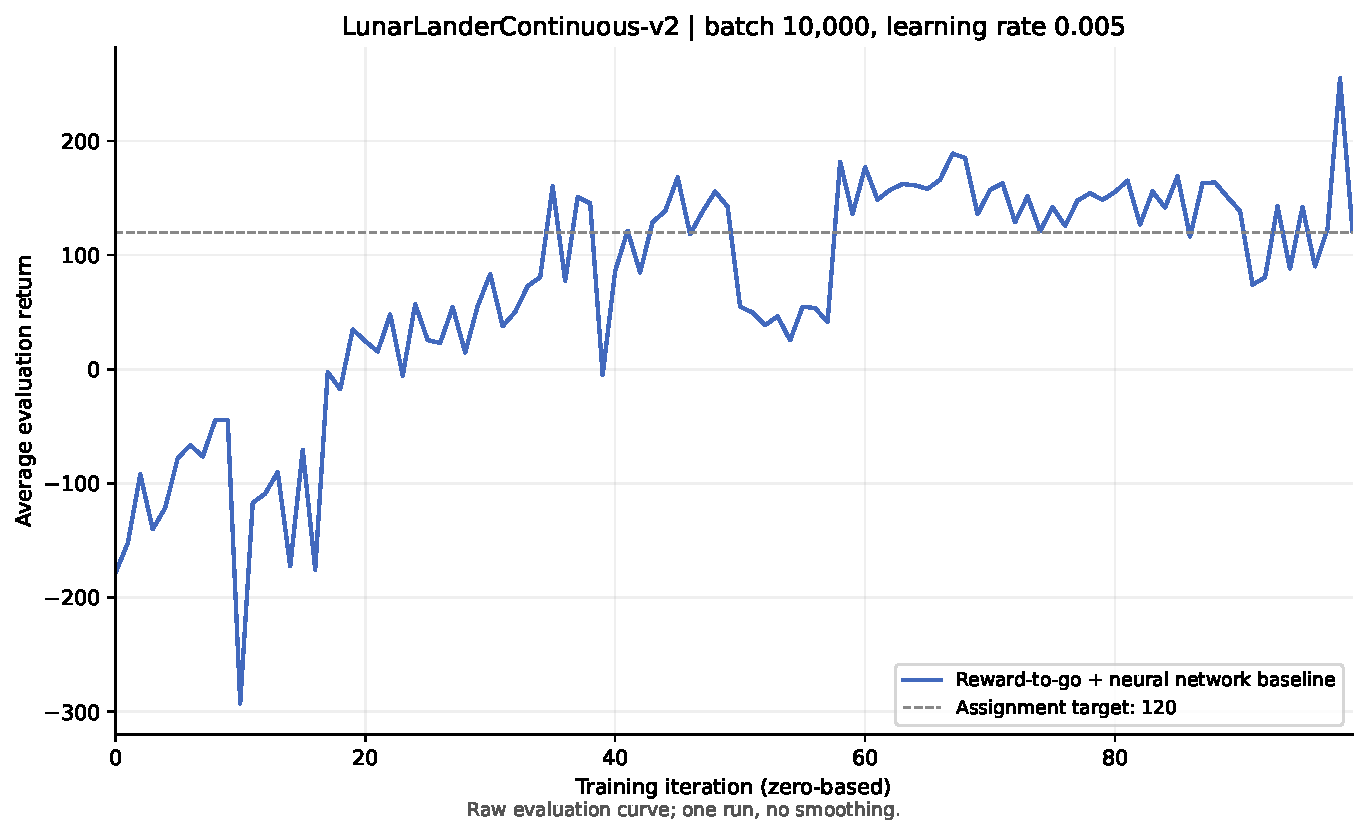
\includegraphics[height=8cm]{results/q3/q3_lunarlander.pdf}
\par\small Final evaluation return: 121.18; mean over the last 10 iterations: 125.53.
\end{answer}

\subsection{Experiment 4 (HalfCheetah) -- \lbrack3.5 points\rbrack}

\subsubsection{Configurations}
\begin{answer}[title=Q7.2.1,height=10cm,width=\linewidth]
\begin{minted}[framesep=2mm, fontsize=\scriptsize, breaklines]{bash}
# CPU runs, seed 1 (default); one thread per process.
export OMP_NUM_THREADS=1 MKL_NUM_THREADS=1 OPENBLAS_NUM_THREADS=1
for b in 10000 30000 50000; do
  for r in 0.005 0.01 0.02; do
    python -m rob831.scripts.run_hw2 --env_name HalfCheetah-v4 \
      --ep_len 150 --discount 0.95 -n 100 -l 2 -s 32 \
      -b "$b" -lr "$r" -rtg --nn_baseline --no_gpu \
      --exp_name "q4_search_b${b}_lr${r}_rtg_nnbaseline"
  done
done
\end{minted}
All nine combinations were run. The selected pair maximizes the mean
raw evaluation return over the last 10 iterations; each configuration
uses one seed. The loops list the commands; jobs were executed concurrently.
\end{answer}

\subsubsection{Plot -- \lbrack1 points\rbrack}
\begin{answer}[title=Q7.2.2,height=10cm,width=\linewidth]
\centering
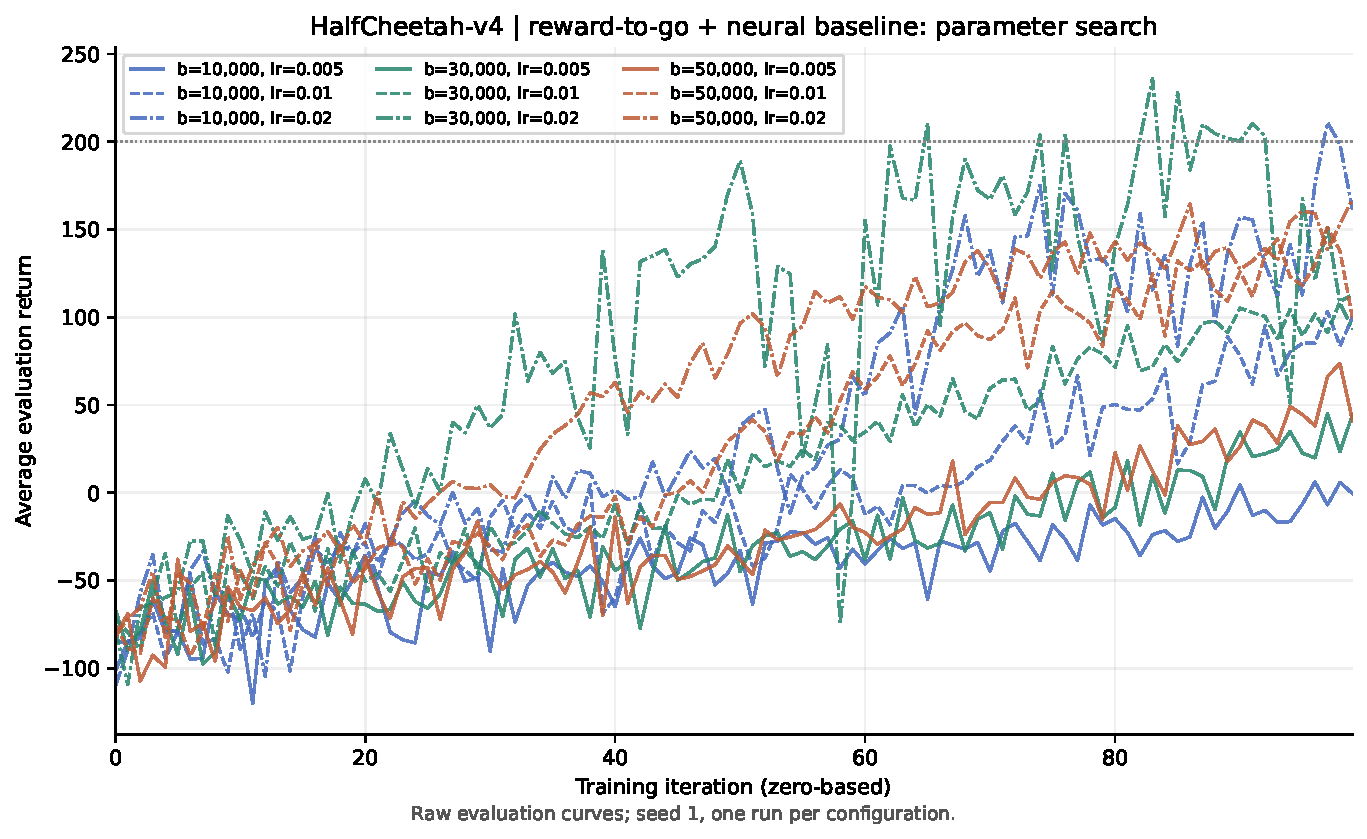
\includegraphics[height=8cm]{results/q4/q4_search.pdf}
\end{answer}

\subsubsection{ Optimal b* and r* -- \lbrack0.5 points\rbrack}
\begin{answer}[title=Q7.2.3,height=4cm,width=\linewidth]
The selected pair is $\mathbf{b^*=10000}$ and $\mathbf{r^*=0.02}$.
It has the highest mean evaluation return over the last 10 iterations
(155.60) among the nine tested configurations, compared with 141.57 for
$b=30000,r=0.02$ and 146.41 for $b=50000,r=0.02$.
Its peak evaluation return is 210.90 and final return is 161.29;
it does not maintain the target of 200 by the end of this seed-1 run.
\end{answer}

\subsubsection{ Plot -- \lbrack0.5 points\rbrack}
\begin{answer}[title=Q7.2.4,height=10cm,width=\linewidth]
\centering
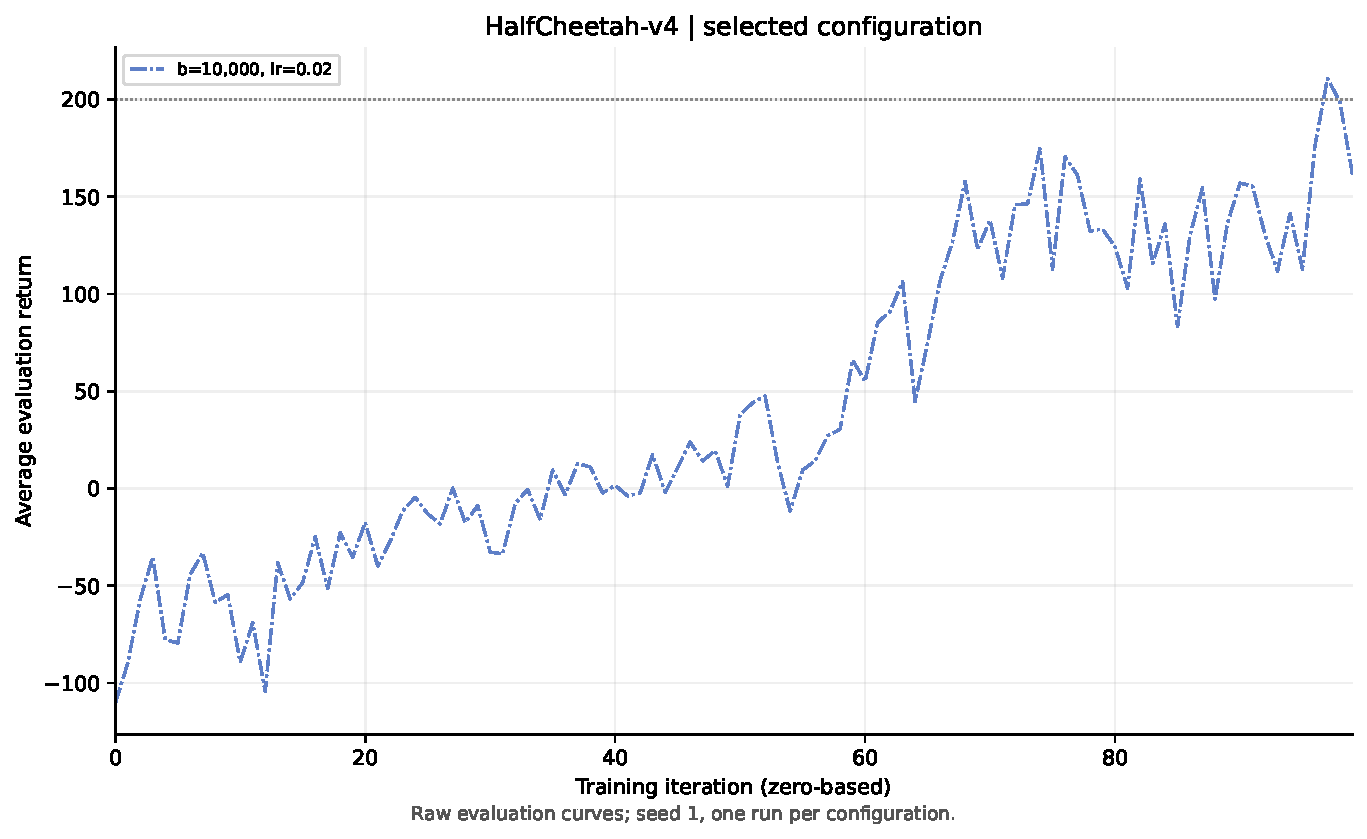
\includegraphics[height=8cm]{results/q4/q4_best.pdf}
\end{answer}

\subsubsection{ Describe how b* and r* affect task performance -- \lbrack0.5 points\rbrack}
\begin{answer}[title=Q7.2.5,height=4cm,width=\linewidth]
\small
Increasing the learning rate improved the last-10 mean at every batch size.
For $b=10000$, rates 0.005, 0.01, and 0.02 gave $-5.37$, 83.98, and 155.60;
thus 0.005 learned too slowly over these 100 updates.
Larger batches helped at smaller rates: at $r=0.01$, the means increased
from 83.98 to 100.46 to 127.74 as $b$ increased.
However, at $r=0.02$, the means were 155.60, 141.57, and 146.41, so
larger batches did not improve the selection metric.
More samples can reduce gradient noise but cost more environment interactions
per update. These are empirical, single-seed results; larger batches are not
guaranteed to improve final return.
\end{answer}

\subsubsection{Configurations with optimal b* and r* -- \lbrack0.5 points\rbrack}
\begin{answer}[title=Q7.2.6,height=6cm,width=\linewidth]
\begin{minted}[framesep=2mm, fontsize=\scriptsize, breaklines]{bash}
python -m rob831.scripts.run_hw2 --env_name HalfCheetah-v4 --ep_len 150 \
  --discount 0.95 -n 100 -l 2 -s 32 -b 10000 -lr 0.02 --no_gpu \
  --exp_name q4_b10000_r0.02
python -m rob831.scripts.run_hw2 --env_name HalfCheetah-v4 --ep_len 150 \
  --discount 0.95 -n 100 -l 2 -s 32 -b 10000 -lr 0.02 --no_gpu -rtg \
  --exp_name q4_b10000_r0.02_rtg
python -m rob831.scripts.run_hw2 --env_name HalfCheetah-v4 --ep_len 150 \
  --discount 0.95 -n 100 -l 2 -s 32 -b 10000 -lr 0.02 --no_gpu --nn_baseline \
  --exp_name q4_b10000_r0.02_nnbaseline
python -m rob831.scripts.run_hw2 --env_name HalfCheetah-v4 --ep_len 150 \
  --discount 0.95 -n 100 -l 2 -s 32 -b 10000 -lr 0.02 --no_gpu -rtg \
  --nn_baseline --exp_name q4_b10000_r0.02_rtg_nnbaseline
\end{minted}
\end{answer}

\subsubsection{Plot for four runs with optimal b* and r* -- \lbrack0.5 points\rbrack}
\begin{answer}[title=Q7.2.7,height=10cm,width=\linewidth]
\centering
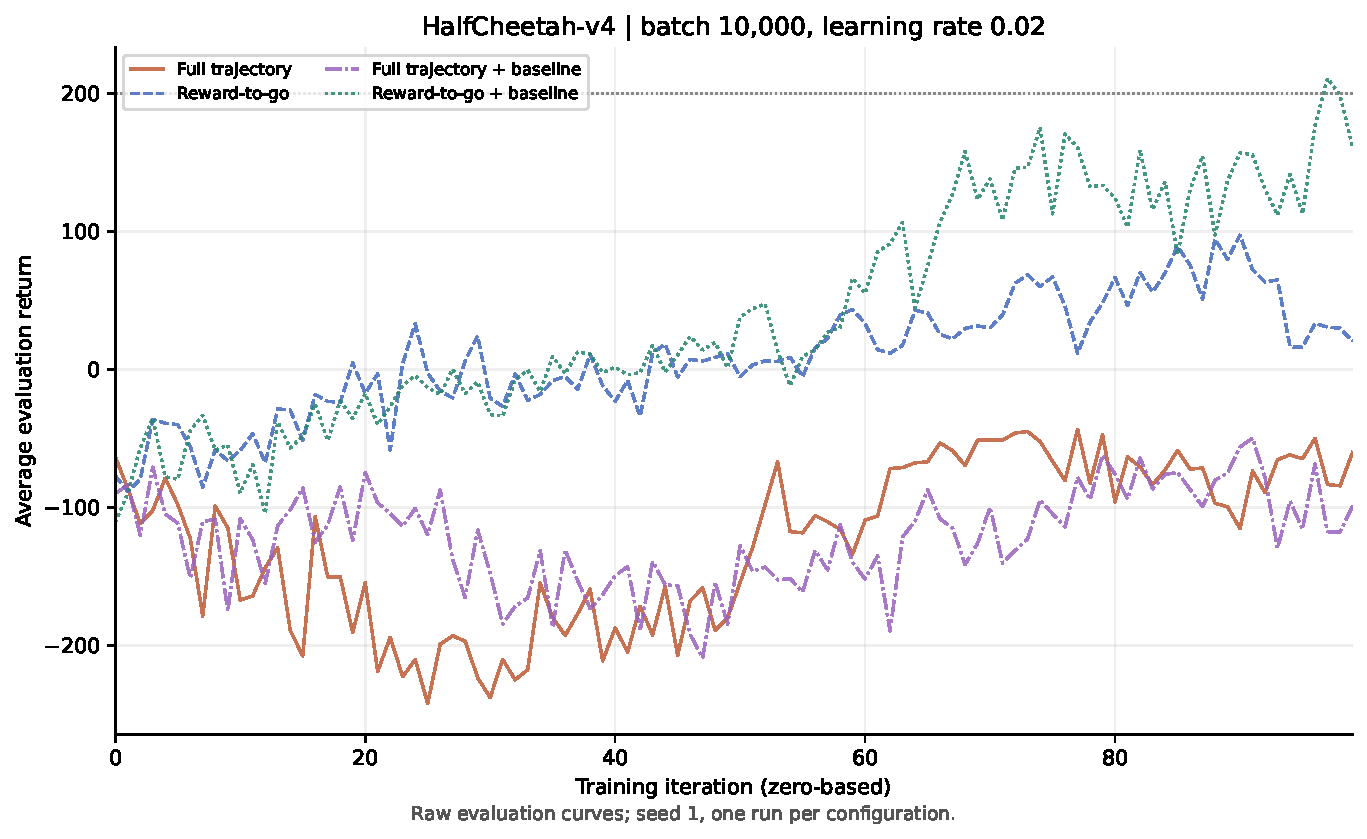
\includegraphics[height=8cm]{results/q4/q4_ablation.pdf}
\par\small Last-10 means (full trajectory / reward-to-go / baseline / both):
$-74.79$ / $44.50$ / $-92.78$ / $155.60$.
\end{answer}

\section{Implementing Generalized Advantage Estimation (3 Pts)}

\subsection{Experiment 5 (Hopper) -- \lbrack3 points\rbrack}

\subsubsection{Configurations}
\begin{answer}[title=Q8.1.1,height=4cm,width=\linewidth]
\begin{minted}[framesep=2mm, fontsize=\scriptsize, breaklines]{bash}
for lam in 0 0.95 0.99 1; do
  python -m rob831.scripts.run_hw2 --env_name Hopper-v4 --ep_len 1000 \
    --discount 0.99 -n 300 -l 2 -s 32 -b 2000 -lr 0.001 \
    --reward_to_go --nn_baseline --action_noise_std 0.5 --no_gpu \
    --gae_lambda "$lam" --exp_name "q5_b2000_r0.001_lambda${lam}"
done
\end{minted}
\end{answer}

\subsubsection{Plot -- \lbrack1 points\rbrack}
\begin{answer}[title=Q8.1.2,height=10cm,width=\linewidth]
\centering
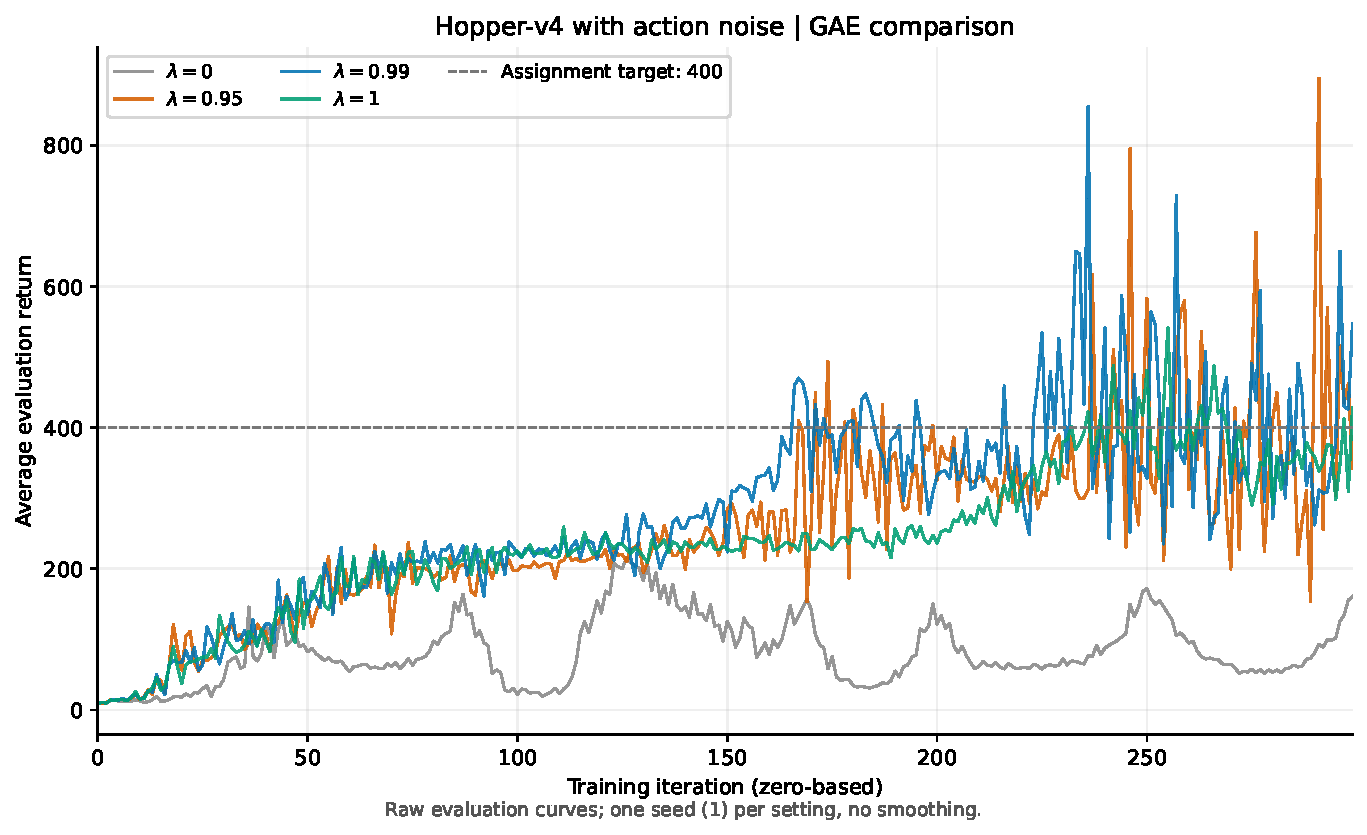
\includegraphics[height=8cm]{results/q5/q5_hopper.pdf}
\end{answer}

\subsubsection{Describe how $\lambda$ affects task performance -- \lbrack1.5 points\rbrack}
\begin{answer}[title=Q8.1.3,height=4cm,width=\linewidth]
\small
The last-10-iteration mean evaluation returns for $\lambda=0,0.95,0.99,1$
were 113.93, 471.31, 396.79, and 359.30, respectively.
Thus $\lambda=0.95$ performed best over this window, while $0.99$ had the
highest last-50 mean (393.10 versus 386.88 for $0.95$).
Both intermediate values achieved performance near or above the target of 400.
A small $\lambda$ relies heavily on the learned value function: lower variance,
but more bias from value errors. Larger $\lambda$ uses longer reward sequences,
reducing this bias at the cost of higher variance; $\lambda=1$ recovers the
Monte Carlo baseline estimator. These single-seed, noisy curves favor an
intermediate tradeoff, with the ranking depending on the evaluation window.
\end{answer}

\subsubsection{Find one robotics paper from the last 5 years that uses policy gradients or an actor-critic method as part of its methodology. 
    In a short paragraph (4--5 sentences): (i) cite the paper, (ii) briefly describe the robot task and how reinforcement learning is used, and (iii) identify one technique from this homework (e.g., reward-to-go, a value-function baseline, or GAE) that is related to the method used in the paper. A few sentences is enough; this is not meant to be an extensive literature review  -- \lbrack0.5 points\rbrack
}
\begin{answer}[title=Q8.1.4,height=4cm,width=\linewidth]
\footnotesize
Miki et al., ``Learning robust perceptive locomotion for quadrupedal robots
in the wild,'' \textit{Science Robotics} 7(62), 2022
(\url{https://arxiv.org/abs/2201.08117})

The task is to follow velocity commands over challenging terrain using
onboard proprioceptive and terrain observations.
They train a teacher policy in simulation with Proximal Policy Optimization
(PPO), giving it privileged terrain and robot information.
A student policy then learns to imitate the teacher from noisy observations
and is deployed on the real robot.
Their PPO training uses generalized advantage estimation with $\lambda=0.95$
(Supplementary Table S1), connecting the method to our Hopper experiment
and its bias--variance tradeoff in advantage estimation.
\end{answer}

\end{document}
